%%% TODO This was CHATGPT generated and looks like shit %%%

\documentclass{standalone}
\usepackage{tikz}

\begin{document}
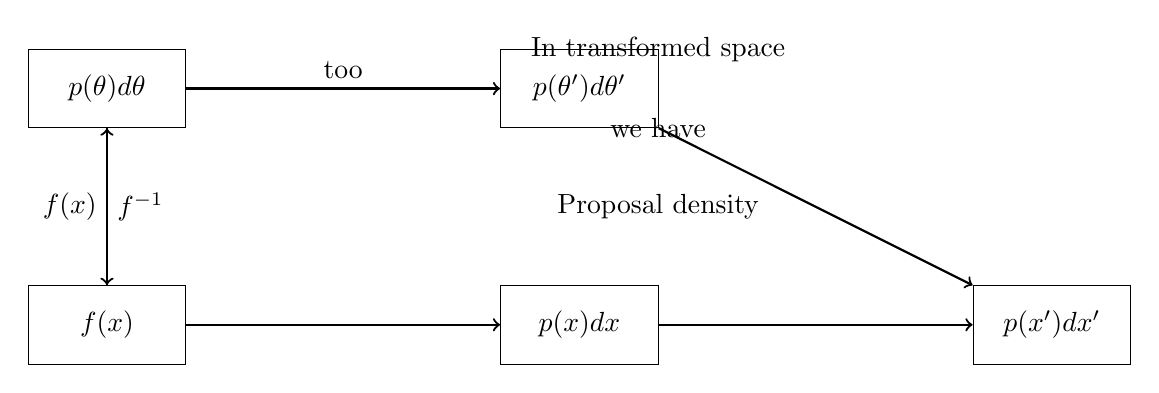
\begin{tikzpicture}
    % Node styles
    \tikzstyle{prob} = [rectangle, draw, minimum width=2cm, minimum height=1cm]
    \tikzstyle{arrow} = [->,thick]

    % Nodes
    \node (p_theta) at (0, 3) [prob] {$p(\theta)d\theta$};
    \node (p_theta_prime) at (6, 3) [prob] {$p(\theta')d\theta'$};
    \node (f_x) at (0, 0) [prob] {$f(x)$};
    \node (p_x) at (6, 0) [prob] {$p(x)dx$};
    \node (p_x_prime) at (12, 0) [prob] {$p(x')dx'$};

    % Arrows
    \draw[arrow] (p_theta) -- node[anchor=south] {too} (p_theta_prime);
    \draw[arrow] (p_theta) -- node[anchor=east] {$f(x)$} (f_x);
    \draw[arrow] (f_x) -- node[anchor=west] {$f^{-1}$} (p_theta);
    \draw[arrow] (f_x) -- (p_x);
    \draw[arrow] (p_x) -- (p_x_prime);
    \draw[arrow] (p_theta_prime) -- (p_x_prime);

    % Labels
    \node at (7, 3.5) {In transformed space};
    \node at (7, 2.5) {we have};
    \node at (7, 1.5) {Proposal density};

\end{tikzpicture}
\end{document}
